\newpage % Rozdziały zaczynamy od nowej strony.
\section{Heurystyki}

\subsection{Definicja i rola heurystyk}
\indent\ Termin "heurystyka" pochodzi od greckiego \emph{heurískō}, co oznacza \emph{znajdować/odkrywać} \cite{heuristicEtymology}. Heurystyki to uproszczone metody podejmowania decyzji, które umożliwiają szybkie i efektywne rozwiązywanie problemów.

Badania nad heurystykami zostały rozpoczęte przez psychologów Amosa Tversky'ego oraz Daniela Kahnemana w latach 70 XX wieku. Opisane przez nich heurystyki stanowiły wytłumaczenie dla systematycznych odstępstw od teoretycznie bardziej racjonalnych decyzji. Podczas podejmowania decyzji ludzie stosują skróty myślowe, które ułatwiają im podjęcie decyzji, ale jednocześnie sprawiają że są bardziej podatni na błędy poznawcze (ang. cognitive bias). Tversky i Kahneman sformułowali wiele heurystyk używanych w psychologii do dziś, między innymi heurystyki dostępności, zakotwiczenia i dostosowania czy reprezentatywności \cite{tversky74} \cite{psychol} \cite{laibson}.

Przykłady heurystyk:
\begin{itemize}
    \item{\textbf{Dostępności}}: Oceniamy prawdopodobieństwo zdarzenia, na podstawie tego jak łatwo możemy przywołać odpowiednie przykłady. Jeśli jakieś zdarzenie lub informacja jest bardziej dostępna w naszej pamięci, mamy tendencję do przeceniania jej prawdopodobieństwa wystąpienia \cite{tversky74}.
    \item{\textbf{Zakotwiczenia i dostosowania}}: Przy podejmowaniu decyzji polegamy na początkowej informacji (zakotwiczeniu), ale nie dostosowujemy wagi tej informacji po otrzymaniu nowych danych. Przykładem może być sytuacja, gdy konsument początkowo widzi wysoką cenę produktu. Jeśli następnie zobaczy obniżkę, pomyśli że jest to bardzo korzystna oferta. W przeciwnej sytuacji, jeśli najpierw zobaczy przeceniony produkt, a następnie w normalnym wariancie cenowym, będzie wydawał mu się zbyt drogi \cite{tversky74, pricing}.
    \item{\textbf{Reprezentatywności}}: Na podstawie stereotypu, oceniamy prawdopodobieństwo przynależności osoby do danej grupy. Przykładowo: jeśli widzimy zgarbionego, bladego chłopaka w okularach i zostaniemy zapytani czy bardziej prawdopodobne jest to czy jest informatykiem czy rolnikiem, wybierzemy pierwszą opcję. Z logicznego punktu widzenia nie jest to dobry wybór, ponieważ na świecie jest więcej rolników niż informatyków. Dzieje się tak, ponieważ wymienione cechy pasują do istniejącego w naszej głowie stereotypu \cite{tversky74} \cite{sudeep}.
\end{itemize}

\subsection{Heurystyki w grach strategicznych}
W kontekście gier strategicznych, heurystyki są kluczowe dla efektywnego zarządzania zasobami, planowania i adaptacji strategii. Komputerowi przeciwnicy korzystają z heurystyk, aby naśladować ludzkie myślenie i podejmowanie decyzji, co czyni rozgrywkę bardziej wymagającą i interesującą dla graczy.

Przykładowe heurystyki wykorzystywane w grach:
\begin{itemize}
  \item \textbf{Heurystyki oparte na odległości:} Przykładem jest heurystyka najkrótszej ścieżki, która służy do oceny odległości między jednostkami lub celami w grze, co pomaga w planowaniu ruchów i ataków \cite{inproceedings}.
  \item \textbf{Heurystyki oparte na priorytetach:} Pozwalają graczom ustalać priorytety dla różnych celów lub działań. Na przykład, w grach RTS (Real-Time Strategy), przeciwnik może priorytetowo traktować budowanie zasobów lub atakowanie gracza w początkowej fazie gry \cite{Ontan2013ASO}.
  \item \textbf{Heurystyki oparte na doświadczeniu:} Korzystają z wcześniej zdobytych doświadczeń lub wyników gier do podejmowania decyzji. Przykładem może być rozpoznawanie wzorców w ruchach gracza i dostosowywanie strategii na ich podstawie \cite{Weber_Mateas_Jhala_2011}.
\end{itemize}

\subsection{Heurystyki zastosowane w pracy}
\begin{enumerate}
  \item \textbf{Heurystyka maksymalizacji zysku ze strzału} Przeciwnik analizuje ile możliwości ustawienia statków istnieje dla danej komórki. Na rysunku 3.1 widoczna jest mapa prawdopodobieństwa obliczona na podstawie tej heurystyki. Wartości widoczne na każdej komórce oznaczają na ile sposobów można ustawić dostępne statki na danej komórce.  Pola będące krawędziami planszy mają wartość 10, ponieważ może na nich znaleźć się każdy ze statków w pionie i w poziomie, w obu przypadkach w dokładnie jednej pozycji. Pola bliżej środka mają większe wartości, ponieważ statki mogą znajdować się na nich w wielu pozycjach, na przykład poziomy trzymasztowiec może leżeć na polu X, Y na 3 sposoby, poniżej są wymienione jego możliwe współrzędne:
  \begin{itemize}
      \item (X-2,Y), (X-1,Y), (X,Y)
      \item (X-1,Y), (X,Y), (X+1,Y)
      \item (X,Y), (X+1,Y), (X+2,Y)
  \end{itemize}

  Heurystyka maksymalizacji zysku ze strzału pozwala na wykonywanie jak najbardziej efektywnych strzałów pod kątem eliminacji możliwych rozstawień statków.
  
  
  \begin{figure}[!h]
    \label{fig:mapa-prawdopodobienstwa-heurystyka-max-zysku}
    \centering 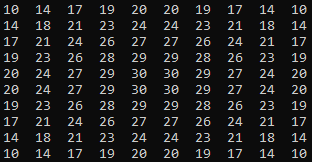
\includegraphics[width=0.5\linewidth]{img/probabilityMapStart.PNG}
    \caption{Mapa prawdopodobieństwa podczas rozpoczęcia gry, przy wykorzystaniu heurystyki maksymalizacji zysku.}
\end{figure}
  
  \item \textbf{Heurystyka najbardziej prawdopodobnej lokalizacji na podstawie trafień}
  Przeciwnik analizuje swoje dotychczasowe trafienia i skupia się na ostrzale komórek sąsiadujących z pojedynczymi trafieniami, oraz wzdłuż linii kilku sąsiadujących trafień. Zatopione statki nie są brane pod uwagę. Jeśli żaden statek nie został jeszcze trafiony, strzały oddawane są losowo. Na rysunku 3.2 widoczne są dwie mapy prawdopodobieństwa. Piersza mapa przedstawia sytuację gdzie trafiona została pojedyncza komórka - wtedy wszystkie sąsiadujące komórki mogą zawierać resztę statku. Na drugim rysunku trafione zostały dwie sąsiadujące komórki - wtedy rozważane są jedynie komórki sąsiadujące, będące na przedłużeniu linii dotychczasowych trafień. Wartości przedstawione na mapie prawdopodobieństwa są umówne - 50 dla komórek sąsiadujących z pojedynczym trafieniem oraz 100 dla komórek sąsiadujących z serią trafień.
  \begin{figure}[!h]
    \label{fig:mapa-prawdopodobienstwa-heurystyka-trafien}
    \centering 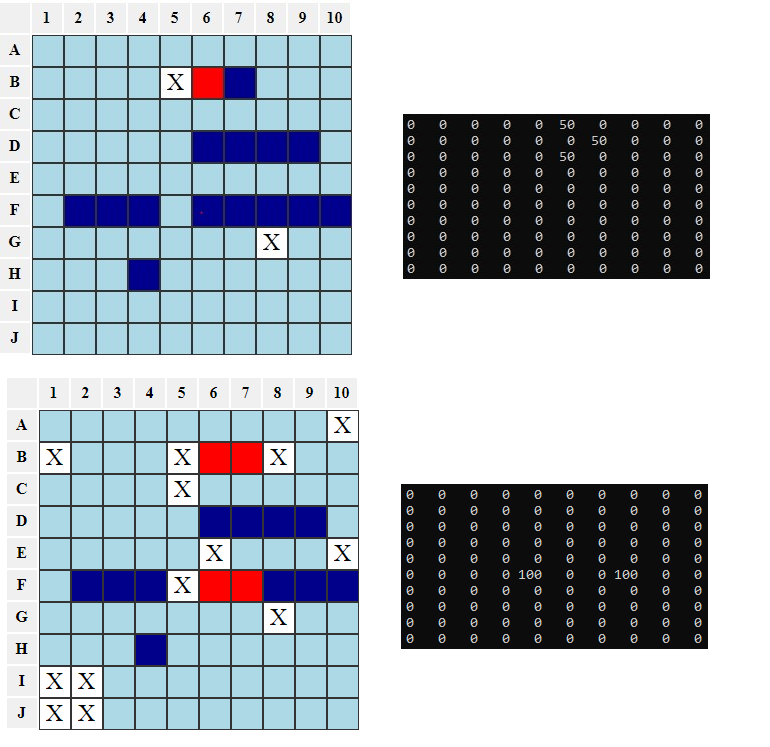
\includegraphics[width=0.9\linewidth]{img/hit-heuristic.png}
    \caption{Mapy prawdopodobieństwa dla dwóch stanów planszy gracza, przy wykorzystaniu heurystyki najbardziej prawdopodobnej lokalizacji na podstawie trafień.}
\end{figure}
  
  \item \textbf{Heurystyka maksymalizacji zysku priorytetyzująca dłuższe statki} Bardzo podobna do już wspomnianej heurystyki maksymalizacji zysku, z jedną różnicą - priorytetyzowane są dłuższe statki. W podstawowej wersji heurystyki jeśli statek mógł znajdować się na komórce (X,Y) w liczbie Z pozycji, dodawaliśmy Z do tej komórki na mapie prawdopodobieństwa. Teraz dodajemy
  \begin{align*}
    Z * L^2
\end{align*}
Gdzie L to długość statku.
  \\ Heurystyka ta pozwala na szybszą eliminację dużych statków.
    \begin{figure}[!h]
    \label{fig:mapa-prawdopodobienstwa-max-zysku-wazona}
    \centering 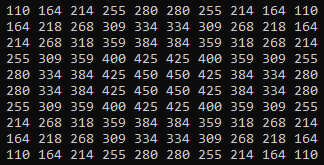
\includegraphics[width=0.5\linewidth]{img/max-benefit-weighted.PNG}
    \caption{Mapa prawdopodobieństwa podczas rozpoczęcia gry, przy wykorzystaniu heurystyki maksymalizacji zysku priorytetyzującej dłuższe statki.}
    \end{figure}

  \item \textbf{Heurystyka maksymalizacji zysku oraz najbardziej prawdopodobnej lokalizacji na podstawie trafień} Połączenie heurystyki maksymalizacji zysku ze strzału (1) oraz heurystyki najbardziej prawdopodobnej lokalizacji na podstawie trafień (2). Ulepszenie podstawowej heurystyki najbardziej prawdopodobnej lokalizacji na podstawie trafień - zamiast losowo ostrzeliwać pola, gdy żadne nie jest jeszcze trafione, teraz strzały oddawane są w pola, które wskazuje heurystyka maksymalizacji zysku. Wagi obu heurystyk są tak dopasowane, aby heurystyka dotychczasowych trafień miała większy wpływ na wybór komórki do ostrzału.

    \begin{figure}[!h]
    \label{fig:mapa-prawdopodobienstwa-heurystyka-laczona}
    \centering 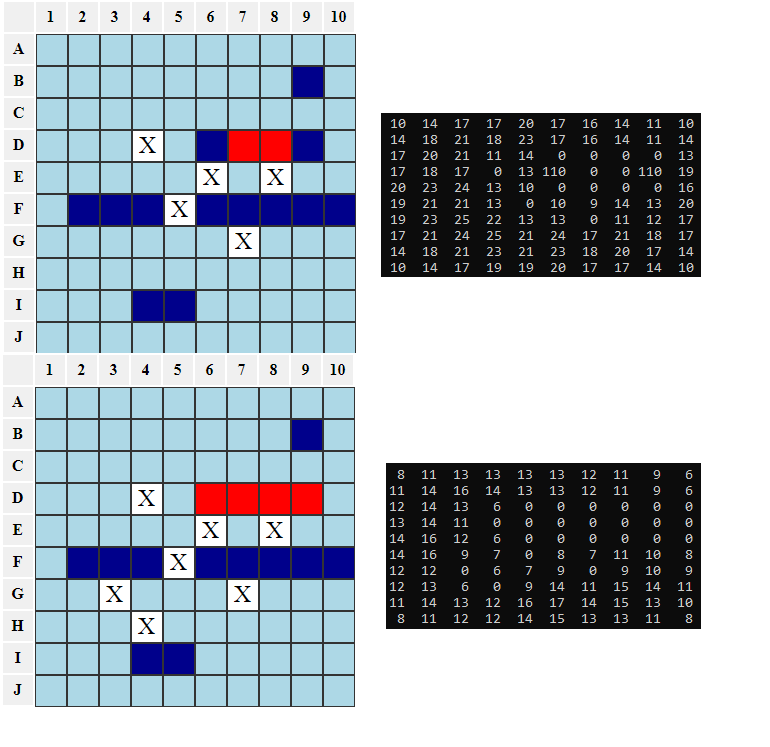
\includegraphics[width=0.9\linewidth]{img/complete-heuristic.png}
    \caption{Mapa prawdopodobieństwa podczas rozpoczęcia gry, przy wykorzystaniu heurystyki maksymalizacji zysku oraz najbardziej prawdopodobnej lokalizacji na podstawie trafień.}
    \end{figure}

  \item \textbf{Heurystyka maksymalizacji zysku oraz najbardziej prawdopodobnej lokalizacji na podstawie trafień priorytetyzująca dłuższe statki} Połączenie heurystyki maksymalizacji zysku ze strzału ważonej (3) oraz heurystyki najbardziej prawdopodobnej lokalizacji na podstawie trafień (2). Wagi obu heurystyk są tak dopasowane, aby heurystyka dotychczasowych trafień miała większy wpływ na wybór komórki do ostrzału. W sytuacji, gdy żadne pole nie jest jeszcze trafione, priorytetyzowane są komórki, które mogą być położeniem najdłuższych statków.
\end{enumerate}